\section{``常量指针''与``指向常量的指针''}
我们在前面讲基本数据类型时,曾经用 \lstinline@const@ 限定符来标记一个变量,使之成为常量;或用 \lstinline@constexpr@ 限定符来标记一个变量,使之成为常量表达式。\par
既然指针也是``变量''的一种,那么我们能否用 \lstinline@const@ 或 \lstinline@constexpr@ 来把它们变成常量或常量表达式呢?\par
先说结论:我们可以使用 \lstinline@const@,将指针限定为``常量指针''或者``指向常量的指针''乃至``指向常量的常量指针''。但是我们不能定义成 \lstinline@constexpr@,因为编译器是不可能未卜先知,知道某个变量在运行时的地址。\par
那么什么是常量指针,什么是指向常量的指针呢?本节就来介绍这两个概念。\par
当我们拿到一个没有任何限制的指针时,我们可以对它的指向进行修改——也就是修改这个指针所存储的地址值;我们还可以通过取内容运算符 \lstinline@*@ 来对它的内容进行修改——也就相当于修改对应变量的值,而修改之后这个指针依然指向原来的位置。如图5.8所示。\par
\begin{figure}[htbp]
    \centering
    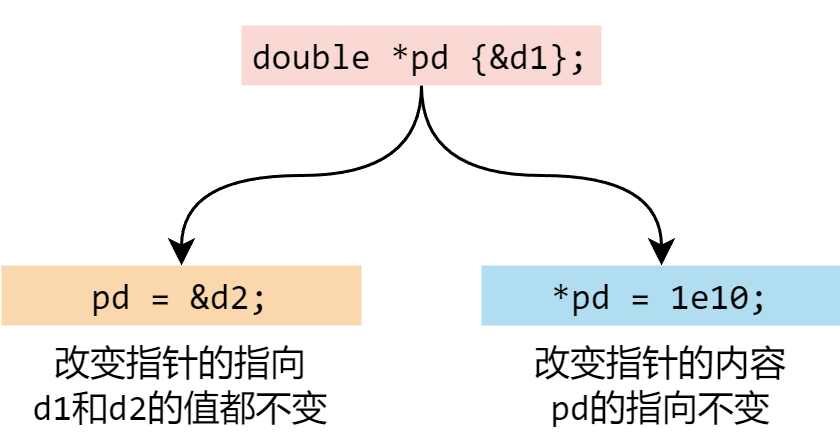
\includegraphics[width=0.6\textwidth]{../images/generalized_parts/05_change_pointer_s_address_or_content_300.png}
    \caption{修改指针的指向/修改指针的内容}
\end{figure}
我们可以通过 \lstinline@const@ 来限制指针的一部分修改能力,从而将其变为常量指针或指向常量的指针。为了避免在代码上出现误解和混淆,我先介绍概念。\par
\begin{itemize}
    \item \textbf{常量指针(Constant pointer)}限制了指针改变指向的能力。这种指针一经初始化,就不能改变指向。但是这不影响我们可以修改它的内容。
    \item \textbf{指向常量的指针(Pointer to constant,简称指针常量\footnote{笔者十分不推荐使用``指针常量''这个名字!它极易与常量指针混淆。})}限制了指针改变内容的能力。我们不能用这种指针来改变内容,但是它可以改变指向。虽然名为``指向常量的指针'',但它也完全可以指向变量。如果它指向变量,那么我们可以用变量名来修改内容;但是不能用这个指针来修改内容。
\end{itemize}
我们还可以用更符号化的表述来阐释它们之间的关系:\par
如果 \lstinline@pd@ 是一个常量指针,那么 \lstinline@pd@ 不能改变;但 \lstinline@*pd@ 是有可能改变的。\par
如果 \lstinline@pd@ 是一个指向常量的指针,那么 \lstinline@*pd@ 不能改变;但 \lstinline@pd@ 是有可能改变的。\par
当你理顺了它们的区别之后,我们就来讲讲怎么用 \lstinline@const@ 限定符来把指针限制成常量指针或指向常量的指针。这是定义的语法:
\begin{lstlisting}
    const int *ptc1; //定义一个指向常量的指针。它可以改变指向,所以无需初始化
    int const *ptc2 {nullptr}; //int与const的位置可互换,也是定义指向常量的指针
    int* const cp {nullptr}; //将const置于*之后,定义一个常量指针,必须初始化
\end{lstlisting}
怎么理解这个定义语法,并把这三种看上去非常相像的语法区分开呢?我们可以这样想:\par
\lstinline@const@ 会对它所标记之物作出限制,使其不能改变。如果 \lstinline@const@ 限制的是 \lstinline@p@,那么 \lstinline@p@ 就不可改变,但 \lstinline@*p@ 可以改变——这正是常量指针的特性;如果 \lstinline@const@ 限制的是 \lstinline@*p@,那么 \lstinline@*p@ 就不可改变,但 \lstinline@p@ 可以改变——这正是指向常量指针的特性。\par
回到我们的定义语法。\lstinline@const int *ptc1@ 这里,我们看,\lstinline@const@ 之后的部分除了 \lstinline@int@(这个不用管)就是 \lstinline@*ptc1@,于是 \lstinline@const@ 直接限定了 \lstinline@*ptc1@,所以 \lstinline@*ptc1@ 不可变,而 \lstinline@ptc1@ 可变,所以它是指向常量的指针;\par
\lstinline@int const *ptc2@ 同理,\lstinline@const@ 直接限定了 \lstinline@*ptc2@,所以 \lstinline@*ptc2@ 不可变,而 \lstinline@ptc2@ 可变,所以它也是指向常量的指针;\par
到了 \lstinline@int* const cp@ 这儿,情况有点不太一样。\lstinline@const@ 直接限定了 \lstinline@cp@,所以 \lstinline@cp@ 不可变,而 \lstinline@cp*@ 仍然可变,所以它是常量指针。\par
图5.9可以帮助你梳理它们之间的区别。\par
\begin{figure}[htbp]
    \centering
    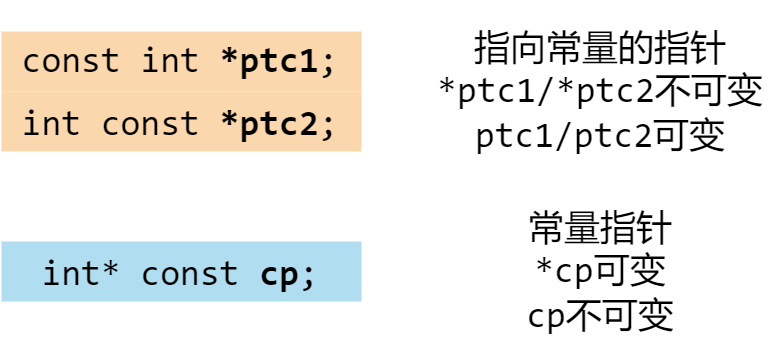
\includegraphics[width=0.7\textwidth]{../images/generalized_parts/05_definition_of_constant_pointer_and_pointer_to_const_300.png}
    \caption{\lstinline@const@ 限制了什么?}
\end{figure}
知道了这个语法规则,那么定义一个``指向常量的常量指针''的语法也就很容易理解了:
\begin{lstlisting}
    const int* const cptc {nullptr}; //定义一个指向常量的常量指针
\end{lstlisting}
在这里,第一个 \lstinline@const@ 限制了 \lstinline@*cptc@ 不能改变,而第二个 \lstinline@const@ 限制了 \lstinline@cptc@ 不能改变,所以这个指针一经定义,既不能改变指向,也不能改变内容。\par
指向常量的指针常见于函数参数,因为很多时候我们需要限制函数对参数的修改能力,确保有些信息是只读的,以免在函数中不小心修改与参数有关的信息。举例来说,\lstinline@cstring@ 库中有 \lstinline@strlen@ 函数,它可以求出一个字符串\footnote{我们会在后面讲到字符串。}的长度。这个函数的声明格式是
\begin{lstlisting}
std::size_t strlen( const char* str );
\end{lstlisting}
这很好理解。既然它只是求算字符串的长度,那么当然没有必要让它具备修改目标字符串的能力,因此直接定义成指向常量的指针就没有潜在风险了。\par
